\section{Auswertung}

Die im Folgenden durchgeführten Regressionsrechnungen werden mit dem
Python Paket \emph{scipy.optimize}\cite{scipy} durchgeführt.

\subsection{Untersuchung der Gegenspannunng für verschieden farbiges Licht}
Die Bremsspannung wird für sechs verschiedene Farben untersucht, es wird
\emph{gelbes}, \emph{grünes}, \emph{blau-grünes}, \emph{violettes} und zwei \emph{ultaviolette}
Lichter untersucht. Erzeugt wird das Licht mit Hilfe einer $\map{Hg}$-Lampe.
Die Messwerte sind in den Tabellen \ref{tab: gelb} - \ref{tab: uv_zwei} aufgelistet.
\begin{table} 
\centering 
\caption{Gemessener Photostrom bei gelbem Licht} 
\label{tab: gelb} 
\begin{tabular}{S S S } 
\toprule  
{Bremsspannung $U$ in $\si{\volt}$} & {Photostrom $I_{\map{p}}$ in $\si{\nano\ampere}$} & {Photostrom $\sqrt{I_{\map{p}}}$ in $\sqrt{\si{\nano\ampere}}$}  \\ 
\midrule  
 0.001  & 0.14  & 0.37\\ 
0.020  & 0.12  & 0.35\\ 
0.041  & 0.10  & 0.32\\ 
0.060  & 0.10  & 0.32\\ 
0.080  & 0.08  & 0.28\\ 
0.100  & 0.07  & 0.26\\ 
0.120  & 0.06  & 0.24\\ 
0.140  & 0.05  & 0.22\\ 
0.160  & 0.04  & 0.20\\ 
0.181  & 0.03  & 0.17\\ 
0.200  & 0.03  & 0.17\\ 
0.220  & 0.02  & 0.14\\ 
0.240  & 0.02  & 0.13\\ 
0.260  & 0.01  & 0.12\\ 
0.280  & 0.01  & 0.10\\ 
0.300  & 0.01  & 0.09\\ 
0.320  & 0.01  & 0.08\\ 
\bottomrule 
\end{tabular} 
\end{table}
\input{../Messdaten/grün.tex}
\input{../Messdaten/grün_blau.tex}
\begin{table} 
\centering 
\caption{Gemessener Photostrom bei violettem licht} 
\label{tab: violett} 
\begin{tabular}{S S S } 
\toprule  
Jo  \\ 
\midrule  
 0.001  & 0.58  & 0.76\\ 
0.102  & 0.48  & 0.69\\ 
0.200  & 0.40  & 0.63\\ 
0.301  & 0.32  & 0.57\\ 
0.401  & 0.24  & 0.49\\ 
0.503  & 0.16  & 0.40\\ 
0.604  & 0.10  & 0.32\\ 
0.702  & 0.06  & 0.24\\ 
0.801  & 0.04  & 0.20\\ 
0.902  & 0.02  & 0.14\\ 
1.001  & 0.01  & 0.10\\ 
1.103  & 0.00  & 0.00\\ 
\bottomrule 
\end{tabular} 
\end{table}
\begin{table} 
\centering 
\caption{Gemessener Photostrom beim ersten ultravioletten licht} 
\label{tab: uv_eins} 
\begin{tabular}{S S S } 
\toprule  
Jo  \\ 
\midrule  
 0.001  & 0.14  & 0.37\\ 
0.101  & 0.12  & 0.35\\ 
0.200  & 0.10  & 0.32\\ 
0.300  & 0.08  & 0.28\\ 
0.401  & 0.08  & 0.28\\ 
0.500  & 0.06  & 0.24\\ 
0.602  & 0.04  & 0.20\\ 
0.701  & 0.03  & 0.17\\ 
0.802  & 0.02  & 0.14\\ 
0.900  & 0.01  & 0.10\\ 
1.001  & 0.01  & 0.10\\ 
1.101  & 0.00  & 0.00\\ 
\bottomrule 
\end{tabular} 
\end{table}
\begin{table} 
\centering 
\caption{Gemessener Photostrom beim zweiten ultravioletten licht} 
\label{tab: uv_zwei} 
\begin{tabular}{S S S } 
\toprule  
Jo  \\ 
\midrule  
 0.020  & 1.00  & 1.00\\ 
0.100  & 0.90  & 0.95\\ 
0.200  & 0.90  & 0.95\\ 
0.400  & 0.60  & 0.77\\ 
0.600  & 0.50  & 0.71\\ 
0.800  & 0.30  & 0.55\\ 
1.000  & 0.20  & 0.45\\ 
1.200  & 0.10  & 0.32\\ 
1.400  & 0.04  & 0.20\\ 
1.600  & 0.01  & 0.10\\ 
1.800  & 0.00  & 0.00\\ 
\bottomrule 
\end{tabular} 
\end{table}
An die gemessenen Spannungen $U$ und an die Wurzel des Photostroms $I\ua{p}$ wird eine
Regressionsgerade
\begin{equation}
  \label{eq:reg}
  g(x)=mx+b
\end{equation}
gefittet.
In den Darstellungen \ref{fig: darstellung_1} bis \ref{fig: darstellung_3} werden die Ergebnisse der Regressionsrechung
illustriert.
\begin{figure}
  \centering
  \begin{subfigure}{0.48\textwidth}
    \centering
    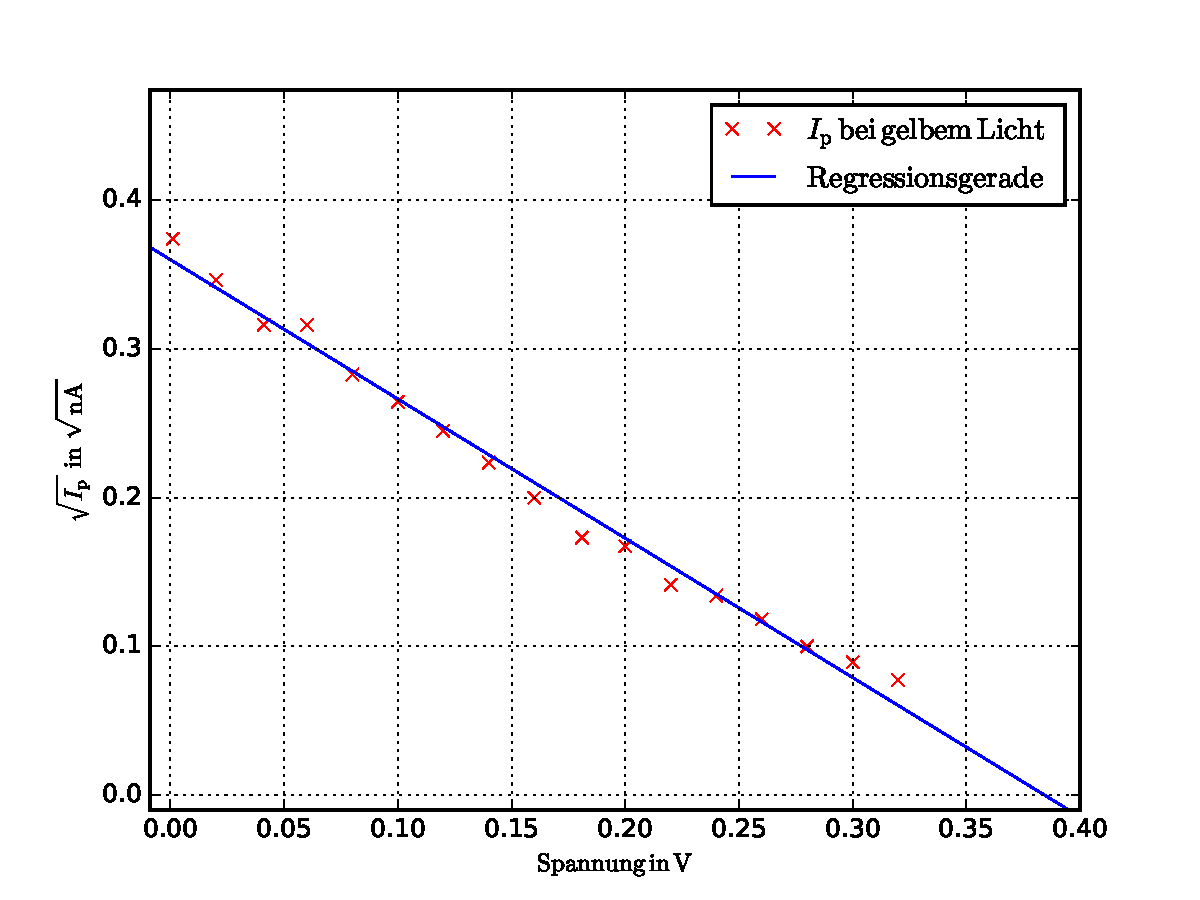
\includegraphics[width=1 \textwidth]{../Messdaten/gelbem.pdf}
    \caption{Gelbes Licht.}
    \label{fig: gelb}
  \end{subfigure}
  \begin{subfigure}{0.48\textwidth}
    \centering
    \includegraphics[width=1 \textwidth]{../Messdaten/grünem.pdf}
    \caption{Grünes Licht.}
    \label{fig: grün}
  \end{subfigure}
  \caption{Darstellung der linearen Abhängigkeit von $\sqrt{I\ua{p}}$ zur Bremsspanung $U$.}
  \label{fig: darstellung_1}
\end{figure}
\begin{figure}
  \centering
  \begin{subfigure}{0.48\textwidth}
    \centering
    \includegraphics[width=1 \textwidth]{../Messdaten/grün-blauem.pdf}
    \caption{Grün-blaues Licht.}
    \label{fig: grün-blau}
  \end{subfigure}
  \begin{subfigure}{0.48\textwidth}
    \centering
    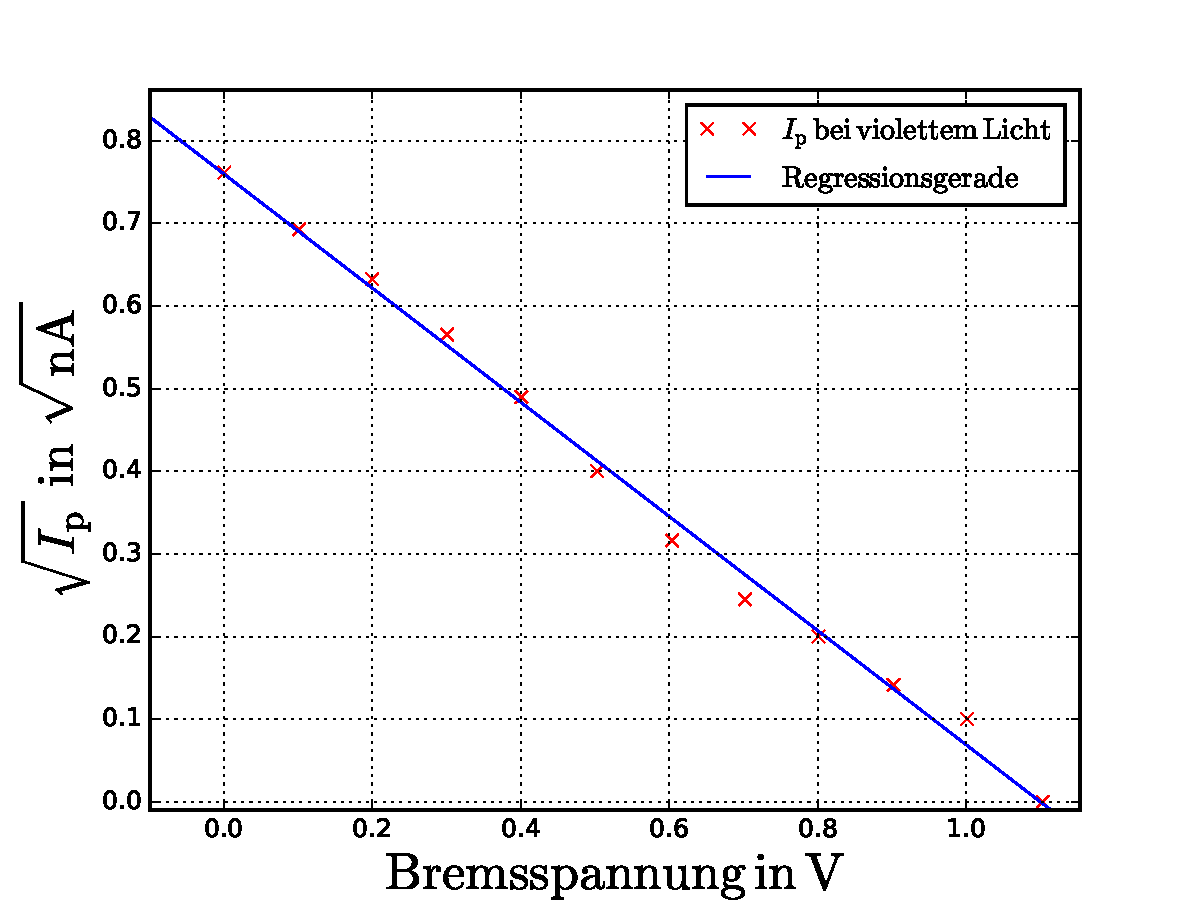
\includegraphics[width=1 \textwidth]{../Messdaten/violettem.pdf}
    \caption{Violettem Licht.}
    \label{fig: violett}
  \end{subfigure}
  \caption{Darstellung der linearen Abhängigkeit von $\sqrt{I\ua{p}}$ zur Bremsspannung $U$.}
  \label{fig: darstellung_2}
\end{figure}
\begin{figure}
  \centering
  \begin{subfigure}{0.48\textwidth}
    \centering
    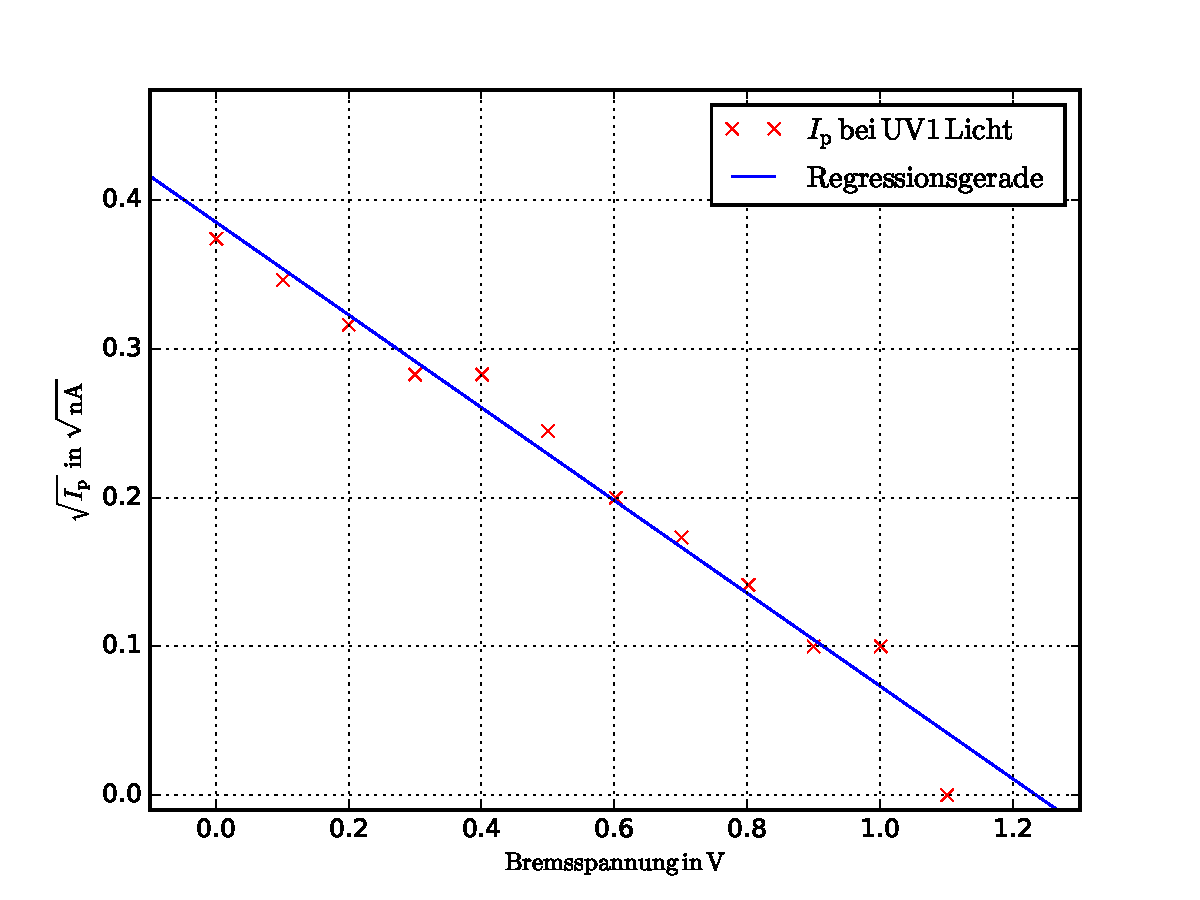
\includegraphics[width=1 \textwidth]{../Messdaten/uv_eins.pdf}
    \caption{UV 1 Licht.}
    \label{fig: uv_eins}
  \end{subfigure}
  \begin{subfigure}{0.48\textwidth}
    \centering
    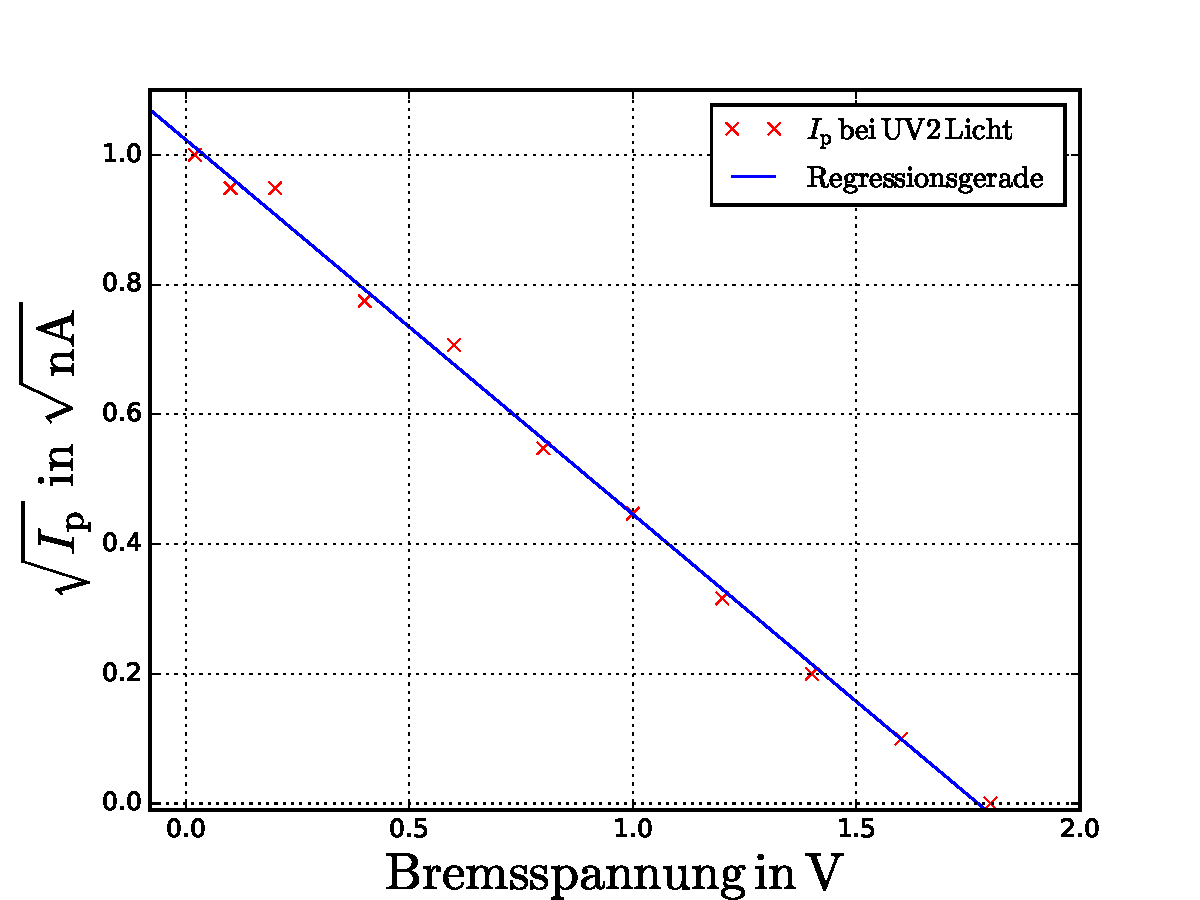
\includegraphics[width=1 \textwidth]{../Messdaten/uv_zwei.pdf}
    \caption{UV 2 Licht.}
    \label{fig: uv_zwei}
  \end{subfigure}
  \caption{Darstellung der linearen Abhängigkeit von $\sqrt{I\ua{p}}$ zur Bremsspannung $U$.}
  \label{fig: darstellung_3}
\end{figure}
Die aus der Ausgleichsrechnung erhaltenden Parameter sind in Tabelle
\ref{tab: messergebnisse} aufgelistet. Die Grenzspannung $U\ua{g}$ wird
wie folgt berechnet:
\begin{equation}
  \label{eq:ug}
  U\ua{g}\overset{\ref{eq:reg}}{=}-\frac{b}{m}.
\end{equation}
\begin{table}
\centering
\caption{Messergebnisse für die verschiedenen Wellenlängen}
\label{tab: messergebnisse}
\begin{tabular}{ S S S S S S S }
\toprule
 {Farben} & {$m$ in $\si{\ampere\per\volt}$} & { $\sigma_{\map{m}}$ in $\si{\ampere\per\volt}$ } & { $b$ in $\si{\ampere}$} & { $\sigma_{\map{b}}$ in $\si{\ampere}$} & {$U_{\map{g}}$ in $\si{\volt}$ } & { $\sigma_{U_{\map{g}}}$ in $\si{\volt}$}     \\
\midrule
\text{gelb} &  0.94  & 0.02  & 0.36  & 0.00  & 0.38  & 0.01\\
\text{grün}& -1.36  & 0.05  & 0.60  & 0.01  & 0.44  & 0.02\\
\text{blau-grün}& -0.24  & 0.01  & 0.18  & 0.00  & 0.75  & 0.02\\
\text{violett}& -0.69  & 0.01  & 0.76  & 0.01  & 1.10  & 0.03\\
\text{uv 1} & -0.94  & 0.02  & 0.36  & 0.00  & 1.24  & 0.01\\
\text{uv 2}& -0.58  & 0.01  & 1.02  & 0.01  & 1.77  & 0.04\\
\bottomrule
\end{tabular}
\end{table}


\subsection{Bestimmung von $\frac{\map{h}}{\map{e}}$ und der Austrittsarbeit}

Die im vorangegangenden bestimmten Grenzspanunngen werden im
Folgenden genutzt, um die Konstante $\frac{\map{h}}{\map{e}}$ und die Austrittsarbeit des Kathodenmaterials
experimentell zu bestimmen.
Es wird dazu eine Regressionrechnung für $U\ua{g}(f)$ durchgeführt.
Aus der Versuchsanleitung\cite{anleitung500} werden die Wellenlängen der verschieden Farben der $\map{Hg}$-Lampe (vgl. Tabelle \ref{tab: wellen})
entnommen.
\begin{table}
\centering
\caption{Untersuchtes Lichtspektrum der $\map{HG}$-Lampe }
\label{tab: wellen}
\begin{tabular}{S S S }
\toprule
{Farbe} & {$\lambda$ in \si{\nano\meter}} & { $f$ in $\si{\THz}$ } \\
\midrule
\text{gelb} & 577.0  & 519.6\\
\text{grün} & 546.0  & 549.1\\
\text{blau-grün} & 492.0  & 609.3\\
\text{violett}  & 434.0  & 690.8\\
\text{uv 1}  & 365.0  & 821.3\\
\text{uv 2} & 366.0  & 819.1\\
\bottomrule
\end{tabular}
\end{table}

Die Umrechnung von der Wellenlänge $\lambda$ in die Frequenz $f$ erfolgt mit
\begin{equation*}
  \label{eq:umrech}
  f=\frac{\map{c}}{\lambda}.
\end{equation*}
Hierbei sei $\map{c}$ die Vaakumlichtgeschwindigkeit\cite{scipy}.
Um $\frac{\map{h}}{\map{e}}$ und die Austrittsarbeit $A\ua{k}$ zu bestimmen, wird zunächst die
Gleichung \eqref{eq:regress} umgestellt zu:
\begin{equation*}
  \Leftrightarrow \qquad U\ua{g}=\frac{\map{h}}{\map{e}} f - \frac{A\ua{k}}{\map{e}}.
\end{equation*}
An diese kann eine Regressionsgerade der Form \eqref{eq:reg} gefittet werden.
Der Zusammenhang zwischen Fitparamtern und den gesuchten Größen lautet:
\begin{align*}
  \frac{\map{h}}{\map{e}}&=m\\
  A\ua{k}&=-b \quad \left(\frac{1}{\map{e}}\,\text{liefert die Einheit} \, \si{\eV}\right)
\end{align*}
\begin{figure}
    \centering
    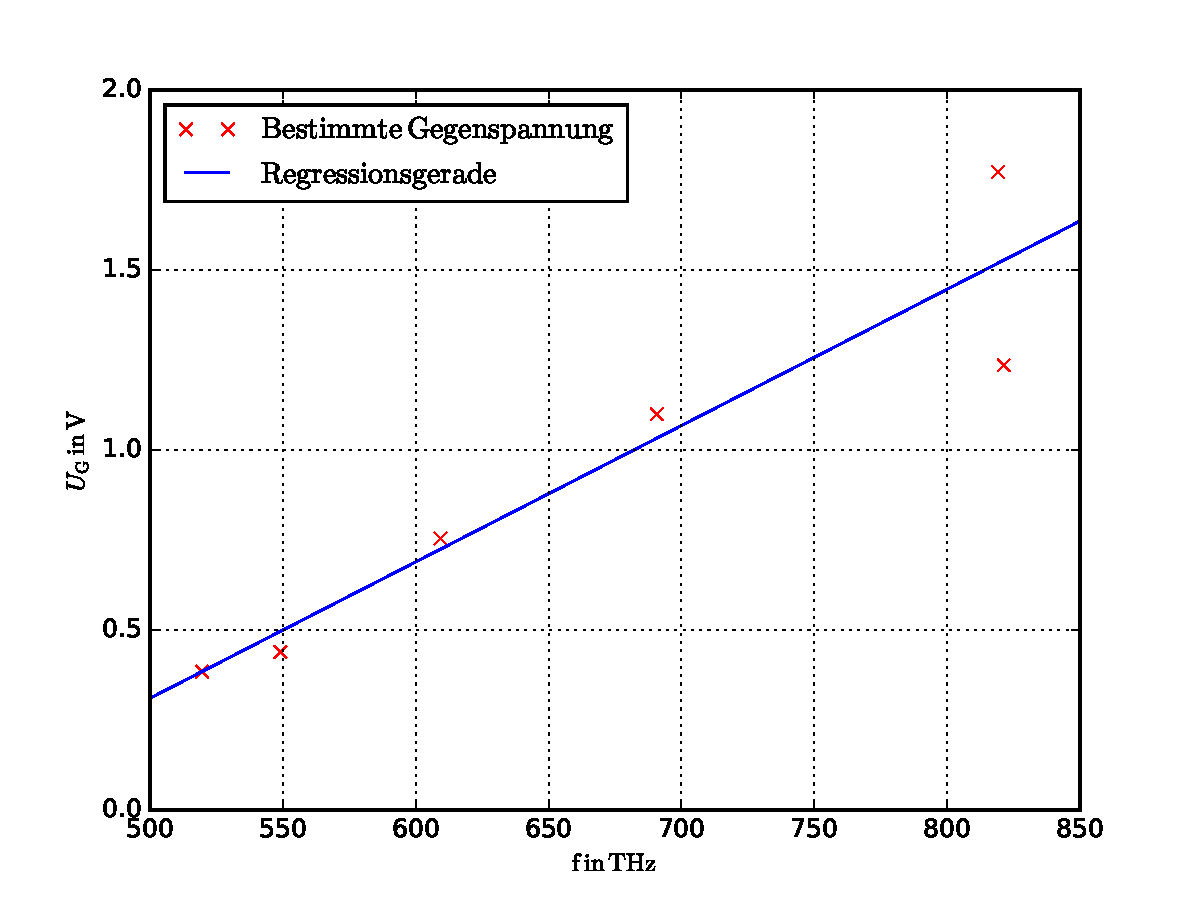
\includegraphics[width=1 \textwidth]{../Messdaten/wellenlaenge_gegen.pdf}
    \caption{Experimentell bestimmten Grenzfrequenzen.}
    \label{fig:grenz}
  \end{figure}
Aus der Regressionsrechnung folgt für die Austrittsarbeit $A\ua{k}$ und die
Konstante $\frac{\map{h}}{\map{e}}$:
\begin{align}
  \label{eq:messergebnisse}
  \begin{aligned}
  \frac{\map{h}}{\map{e}}&= \left(\num{3.8\pm 0.7}\right)\,\num{e-15}\,\si{\eV} \\
  A\ua{k}&=\SI{1.6\pm 0.5}{\eV}.
  \end{aligned}
\end{align}
Die Messwerte und die Regressionsgerade sind in Abbildung \ref{fig:grenz} dargestellt.
\subsection{Untersuchung des Photostroms bei gelbem Licht}
Für die Untersuchung des Photostrom $I\ua{p}$ wurde die
Stromstärke für Spannungen $U$ im Bereich $U\in\left(-20,20\right)\,\si{\volt}$
notiert (vgl. Tab. \ref{tab: gelb_all}).
\begin{table} 
\centering 
\caption{Gemessener Photostrom bei gelbem Licht} 
\label{tab: gelb_all} 
\begin{tabular}{S S } 
\toprule  
{Spanung $U$ in $\si{\volt}$} & {Photostrom $I_{\map{p}}$ in $\si{\nano\ampere}$}  \\ 
\midrule  
 18.970  & 2.100\\ 
18.020  & 2.000\\ 
17.000  & 2.000\\ 
16.010  & 2.100\\ 
15.010  & 2.000\\ 
14.030  & 2.000\\ 
13.000  & 2.000\\ 
12.070  & 2.000\\ 
11.030  & 1.700\\ 
10.070  & 1.700\\ 
9.020  & 1.600\\ 
8.010  & 1.600\\ 
7.000  & 1.500\\ 
6.010  & 1.600\\ 
5.040  & 1.500\\ 
4.000  & 1.400\\ 
3.070  & 1.000\\ 
2.040  & 0.900\\ 
1.010  & 0.600\\ 
0.020  & 0.100\\ 
-0.001  & 0.140\\ 
-0.020  & 0.120\\ 
-0.041  & 0.100\\ 
-0.060  & 0.100\\ 
-0.080  & 0.080\\ 
-0.100  & 0.070\\ 
-0.120  & 0.060\\ 
-0.140  & 0.050\\ 
-0.160  & 0.040\\ 
-0.181  & 0.030\\ 
-0.200  & 0.028\\ 
-0.220  & 0.020\\ 
-0.240  & 0.018\\ 
-0.260  & 0.014\\ 
-0.280  & 0.010\\ 
-0.300  & 0.008\\ 
-0.320  & 0.006\\ 
-0.340  & 0.000\\ 
\bottomrule 
\end{tabular} 
\end{table}
In Abbildung \ref{fig:gelb_all} ist der Stromverlauf dargestellt.
\begin{figure}
    \centering
    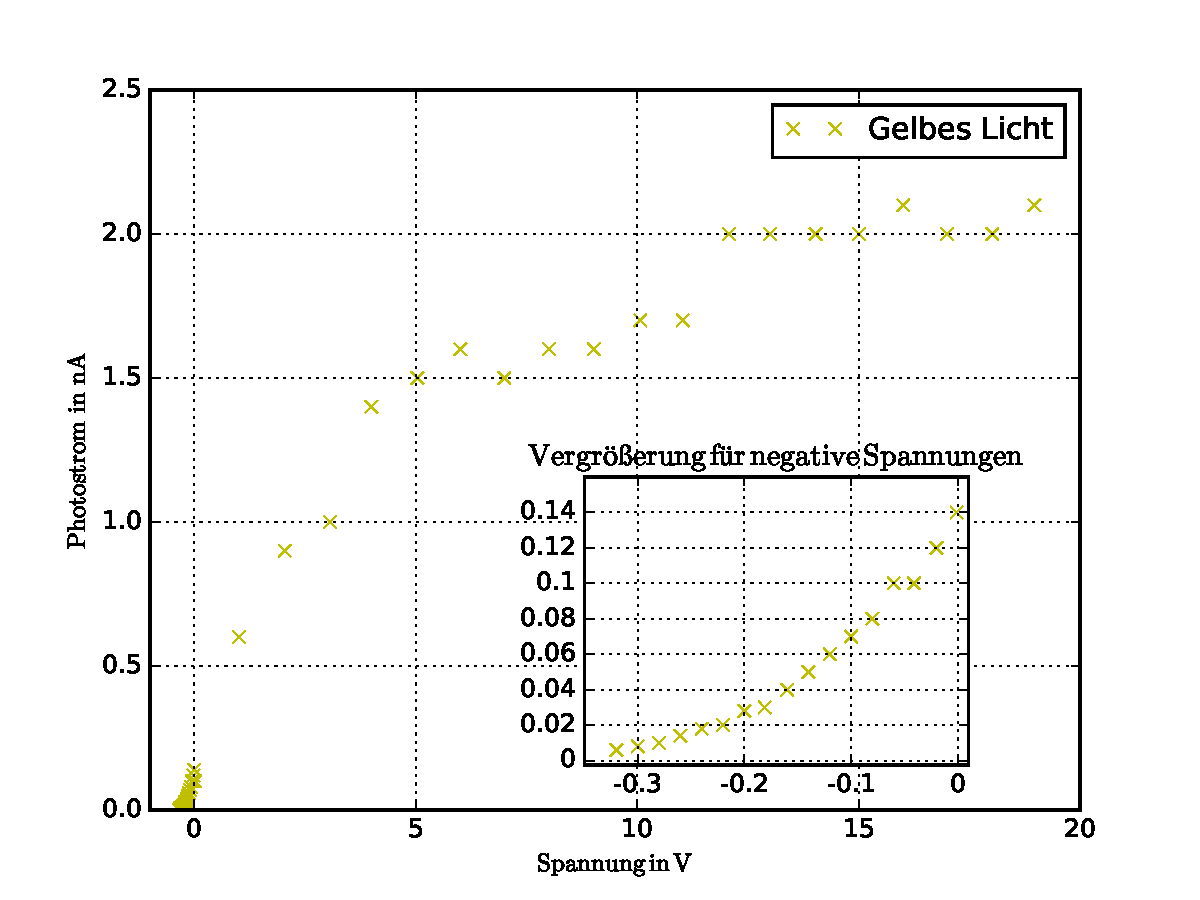
\includegraphics[width=1 \textwidth]{../Messdaten/gelb.pdf}
    \caption{Abhängigkeit des Photostroms von der Spannung.}
    \label{fig:gelb_all}
  \end{figure}.

Die in der Abbildung \ref{fig:gelb_all} zu sehende Sättigung entsteht dadurch, dass
ab einer bestimmten Beschleunigungsspannung alle Elektronen die Anode erreichen.
Lediglich eine Erhöhung der Lichtintensität würde eine Vergrößerung der Stromstärke
zu folge haben.
Das asymptotische Verhalten der Stromstärke ist auf die Anode
bzw. das Streuverhalten der Elektronen zurückzuführen, denn es ist bei der verwendeten
Anode nicht sichergestellt, dass alle Elektronen regrestiert werden.
Das Problem kann zum Beispiel mit einer Anode gelöst werden, die die Photokathode
einhüllt.

Die Stromstärke fällt nicht schlagartig gegen null, da die Elektronen in der Photokathode
eine Energieverteilung besitzen. Auf Grund dessen besitzt nicht jedes ausgelöstes
Elektron dieselbe Energie. Einige Elektronen können dadurch, bis zu einem bestimmten Spannungsbereich,
die Bremsspannung überwinden.

Bei dem Photoeffekt ist auch ein positiver Photostrom beobachtbar, das
Phänomen ist erklärbar damit, dass auch bei der Anode ein lichtelektrischer Effekt
auftritt. Jedoch besitzt die Anode eine höhere Austrittsarbeit, dies sorgt
dafür dass nur einige wenige Elektronen ausgelöst werden.
Verstärkt wird der positive Photostrom durch das Kathoden selber,
denn das Kathodenmaterial verdampft schon für Temperaturen um
$T=\SI{20}{\celsius}$. Das verdampfte Kathodenmaterial kann sich auf die
Anode legen und so die Austrittsarbeit der Anode herabsetzen, folglich steigt der
positive Photostrom.
